\Chapter{A hálón végezhető elemzések}
\Section{Háló korlátosság és puffer kapacitási ellenőrzés}

A háló egy adott helye akkor tekinthető korlátos (\textit{bounded}) helynek, ha bármely jelölésnél a tokenek száma az adott helynél nem megy egy adott korlát fölé. A Petri háló korlátos, ha minden helye korlátos hely.
A háló korlátossága az egyik leggyakoribb és legfontosabb minőségi jellemzője a Petri hálóknak. 

A háló alap tulajdonságainak, beleértve a korlátosságának az elemzésére több módszer is létezik, melyek közül kiemelhető a
\begin{itemize}
\item komponens/elérhetőségi gráf elemzése (SCC),
\item dekompozíciós módszerek.
\end{itemize}

A mátrix reprezentáció esetén transzformációs mátrixok segítségével írják fel a Petri háló dinamikáját. Az alapstruktúra az ú.n. incidencia $M$ mátrixban kerül megadásra, melynek elemei az alábbi jelentéssel bírnak: $A_{ij}=a^+_{ij}-a^-_{ij}$, ahol 
\begin{itemize}
\item $a^+_{ij}: $ az élerősség az i. tranzicióból a j. kimeneti hely felé,
\item $a^-_{ij}$ az élerősség az i. tranzicióhoz a j. bemeneti hely felől.
\end{itemize}

A mátrix alapvetően a tokenek számának a változását mutatja az egyes tranzició átmenetek esetére. A  Petri háló működési alapegyenlete a következő alakban adható meg: 
$$M_k=M_{k-1}+ Au_k,$$
ahol $M_k$ jelöli a háló markereinek (tokenek) státuszát a $k.$ lépésben. Az $u$ vektor a helyek tüzelési státuszt írja le. 

A fenti modellen alapuló elérhetőség vizsgálatok felhasználhatóak a korlátosság elemzésére \cite{murata1989petri}.
A kapcsolódó  egyenletek hatékony, lineáris programozási megoldása szintén ismert \cite{lasserre1989using}.

\Section{Saját modell alaphálóra}

Modellünkben korlátosságnak egy folyam-gráf megközelítését dolgoztuk ki.  A hálóban a következő típusú helyeket definiáljuk:
\begin{itemize}
\item forrás hely,
\item nyelő hely,
\item köztes hely.
\end{itemize}
Feltesszük, hogy csak a köztes helyeken lehet tokeneket tárolni, csak ott vannak pufferek. A hálóban az élekhez egy $I_x$ token áramlás erősséget definiálunk, ahol $x$ jelöli az él indexét. A forrás helyekhez egy $Q_x$ forrás erősség indexet adunk meg. A hálóban az alábbi kapacitás korlátokat vezetjük be:
\begin{itemize}
\item $C_x:$ az $x$. tranzició maximális erőssége,
\item $C_y:$ az $y$. nyelő maximális folyam erőssége.
\end{itemize}

A tranzicióknál a bemenő élek vonatkozásában kétféle működési módot értelmezünk:
\begin{itemize}
\item AND-mód: akkor van tüzelés, ha minden bejövő élnél megvan az al elvárt tokenszám, van szinkron,
\item OR-mód: akkor van tüzelés, ha megjelenik valamely bemeneten egy token, nincs szinkron.
\end{itemize}
A hálóban az alábbi megkötések élnek a folyamerősségekre:
\begin{itemize}
\item forrás helyek esetén: $\sum_y I_y=Q_x$ ($y$: kimenő élek),
\item nyelő helyek esetén: $\sum_y I_y \leq C_x$ ($y$: bejövő élek),
\item belső helyek esetén: 
$\sum_{y(ki)} I_y\leq \sum_{y(be)} I_y$,
\item tranziciók esetén: 
\begin{itemize}
\item $\sum_y I_y\leq C_x$ ($y:$ bejövő élek),
\item $\sum_{y(ki)} I_y = \sum_{y(be)} I_y$,
\item $\forall$ kimenő $x,y$ élre $I_x=I_y$.
\end{itemize}
\end{itemize}
Az AND típusú tranzakciók esetén még ezen felül teljesül, hogy $\forall$ bejövő $x,y$ élre:\\
$I_x = I_y$.

Az egyes belső helyeken a pufferbe áramló tokenek  eredő intentitása:
$$F= \sum_{x(\text{belső hely})} \left( \sum_{y(\text{x bejövő él})} I_y - \sum_{y(\text{x kimenő él})} I_y \right)$$
Az $F$ függvény 0 értéke esetén nincs szükség belső pufferre.

A fenti feladat egy LP programozási feladatnak is tekinthető, ahol a változók az élek $I_x$ nem negatív intenzitásai, és a célfüggvény:
$$F\rightarrow \min$$ alakú.

\Section{Az alkalmazott, kibővített modell színezett hálóra}

A színezett Petri hálók esetén több különböző típusú tokenek élnek a rendszerben. A kapacitás vizsgálatnál ekkor az egyes tranzicióknál eltérő lehet a kapacitás korlát (a maximális folyam erősség) a különböző típusú tokenek esetén. Emiatt külön kell vizsgálni az egyes típusok folyam erősségét, nem lehet összevonni őket.

A színezett hálóban az élekhez $I^c_x$ token áramlás erősségeket definiálunk, ahol $x$ jelöli az él indexét és $c$ a színkód. A forrás helyekhez $Q^c_x$ forrás erősség indexeket adunk meg a különböző $c$ színekre vonatkozólag. A hálóban az alábbi kapacitás korlátokat vezetjük be:
\begin{itemize}
\item $C^C_x$: az $x$. tranzició maximális erőssége a $c$ szín esetén 
\item $C^C_y$: az $y$. nyelő maximális folyam erőssége a $c$ szín esetén
\end{itemize}
A hálóban az alábbi megkötések élnek a folyamerősségekre:
\begin{itemize}
\item forrás helyek ($x$) esetén: $\forall c$ színre: $\sum_{y\text{ kimenő élek}}I^C_Y = Q^C_x$,
\item nyelő helyek ($x$) esetén: $\forall c$ színre: $\sum_{y\text{ bejövő élek}}I^C_y \leq C^C_x$,
\item belső helyek esetén: $\forall c$ színre: $\sum_{y\text{ kimenő élek}} I^C_y \leq \sum_{y\text{ bejövő élek}}$,
\item tranziciók ($x$) esetén:
$$\forall c \text{ színre} \sum_{y\text{ kimenő élek}} I^C_y == \sum_{y\text{ bejövő élek}} I^C_y $$,
$$\sum_{c \text{ színek}}\left( \frac{1}{C^C_x} \left( \sum_{y \text{ bejövő élek}} I^C_y \right) \right) \leq 1$$,
$$\forall c \text{ színre:} \forall \text{ kimenő} (y,z) \text{élre: } I^C_y=I^C_z$$,
\item az AND típusú tranzakciók esetén még ezen felül teljesül, hogy 	$\forall c$ színre: $\forall$ bejövő $(y,z)$ élre $I^C_y=I^C_z$.
\end{itemize}
Az egyes belső helyeken a bufferbe áramló tokenek  eredő intenzitása:
$$F=\sum_{c\text{ színek}} \left( \sum_{x\text{ belső hely}}\left( \sum_{y\text{ bejövő élek }x\text{-nél}}I^C_y - \sum_{y \text{ kimenő helyek }x\text{-nél}} I^C_y \right) \right).$$
Az $F$ függvény 0 értéke esetén nincs szükség belső bufferre. 
A fenti feladat egy lineáris programozási feladatnak (röviden LP) is tekinthető, ahol a változók az élek $I_x$ nem negatív intenzitásai és a célfüggvény $F \rightarrow \min$ alakú. 
\newpage
\Section{A validációs számítás algoritmusa}

A hálót leíró struktúra három alappilléren nyugszik: helyek, tranziciók, élek.

A helyek esetén az alábbi attribútumokat tárolja a rendszer:
\begin{itemize}
\item \texttt{id}: az egyedi azonosító kód,
\item \texttt{inputs}: bejövő élek,
\item \texttt{outputs}: kimenő élek,
\item \texttt{tokens}: tárolt tokenek,
\item \texttt{Q}: forrás intenzitás,
\item \texttt{border}: pozíció jelző, belső vagy határ pozíció.
\end{itemize}        
A tranzíciók jellemzői:
\begin{itemize}
\item \texttt{id}: egyedi azonosító kód,
\item \texttt{inputs}: bejövő élek,
\item \texttt{outputs}: kimenő élek,
\item \texttt{C}: feldolgozási intenzitás,
\item \texttt{mode}: működési mód (AND, OR).
\end{itemize}
Az élek attribútumai:
\begin{itemize}
\item \texttt{id}: azonosító kód,
\item \texttt{input}: induló elem,
\item \texttt{output}: cél elem,
\item \texttt{alfa}: az él kapacitás jelzője,
\item \texttt{inner}: él típusa, belső vagy határ.
\end{itemize}



A program python szegmense később integrálásra került a fő programban. Különböző változásuk után a Goole OR tools lett a végső részmodul, amit erre a célra alkalmaztam. A szintaktikája hasonló a pythonéhoz, de helyenként különbözik. Az előző példa C\# ban a GLOP segítségével megoldva:

A sover létrehozása GLOP-al
\begin{cpp}
Solver solver = Solver.CreateSolver("GLOP");
\end{cpp}
A változókat itt megadhatjuk egy előre definiált tömbbel, vagy egyesével. A programban konverzió miatt az utóbbi lett kiválasztva, mert folyamatosan feltöltető.
\begin{cpp}
Variable weights = solver.MakeNumVar(0.0, int.PositiveInfinity, "weight");
\end{cpp}
Megkötés hozzáadása: példa belső élre
\begin{cpp}
solver.Add(c[2]-c[5]>0);
\end{cpp}
A célfüggvény:
\begin{cpp}
solver.Minimize(i => costs[i] * trVars[i]);
\end{cpp}
Ha kész az előfeltétel, akkor elindítjuk a solvert
\begin{cpp}
Solver.ResultStatus resultStatus = solver.Solve();
\end{cpp}
Itt a result status tartalmazza a megoldást, ha van, ekkor 'OPTIMAL'-al tér vissza, a változók ekkor kinyerhetőek:
\begin{cpp}
sb.Add(c[1].SolutionValue());
\end{cpp}

\Section{Mintafeladat}
Vegyünk egy 4 helyből és 2 tranzicióból álló rendszert. A helyekből egy nyelő, egy forrás és kettő belső hely. A rendszerben 6 él van az ábrán megadott módon. \ref{fig:capactiy}  A gráfban a kerek elem a helyeket, szögletes a tranziciókat jelöli. A csomópont elemben az első jel a hely kódja, a második a kapcsolódó kapacitás érték. A modellben a kisebb indexű tranzició AND tulajdonságú, a másik OR tulajdonságú. 
\begin{figure}[h!]
\centering
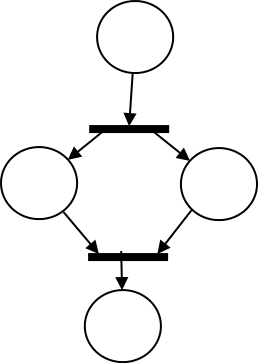
\includegraphics[scale=0.5]{images/capacity.png}
\caption{A mintahálónk}
\label{fig:capactiy}
\end{figure}

A rendszerben 6 (nem negatív) változó jelenik meg:\\
$\{0: Iv_0, 1: Iv_1, 2: Iv_2, 3: Iv_3, 4: Iv_4, 5: Iv_5\}$

Az élek indexelése:
\begin{align*}
0  :  1 \rightarrow 5  \\
1  :  5 \rightarrow 2  \\
2  :  2 \rightarrow 6  \\
3  :  6 \rightarrow 3  \\
4  :  3 \rightarrow 5  \\
5  :  6 \rightarrow 4 
\end{align*}

A rendszerhez az alábbi egyenlőtlenségek kapcsolódnak:

\begin{center}
\begin{tabular}{rll}
$C_1$ &: $Iv_0$ &$= 20$ \\
$C_2$ &: $Iv_1 - Iv_2$ &$\geq 0$\\
$C_3$ &: $Iv_3 - Iv_4$ &$\geq 0$\\
$C_4$ &: $Iv_5$ &$\leq 25$\\
$C_5$ &: $Iv_0 - Iv_1 + Iv_4$ &$= 0$\\
$C_6$ &: $Iv_0 + Iv_4 $&$\leq 50$\\
$C_7$ &: $Iv_0 - Iv_4 $&$= 0$\\
$C_8$ &: $Iv_2 - Iv_3 - Iv_5$&$= 0$\\
$C_9$ &: $Iv_2 $&$\leq 50$\\
$C_{10}$ &: $Iv_3 - Iv_5 $&$= 0$
\end{tabular}
\end{center}

A kapcsolódó célfüggvény:
$$1\cdot Iv_1 + -1\cdot Iv_2 + 1\cdot Iv_3 + -1\cdot Iv_4\rightarrow \min$$.

Az LP feladat megoldható és a kapott megoldás:
\begin{center}
\begin{tabular}{rll}
&$Iv_0$ &: $20.0$\\
&$Iv_1$ &: $40.0$\\
&$Iv_2$ &: $40.0$\\
&$Iv_3$ &: $20.0$\\
&$Iv_4$ &: $20.0$\\
&$Iv_5$ &: $20.0$\\
&$Cost$ & $= 0.0$
\end{tabular}
\end{center}
Tehát a mintarendszerben nincs szükség belső pufferre. 
Ha lecsökkentjük a második tranzició folyamerősségét, az akkor nem kapunk érvényes megoldást. \\
\begin{center}
\begin{tabular}{rll}
&$Iv_0$ &: $10.0$\\
&$Iv_1$ &: $20.0$\\
&$Iv_2$ &: $20.0$\\
&$Iv_3$ &: $10.0$\\
&$Iv_4$ &: $10.0$\\
&$Iv_5$ &: $10.0$
\end{tabular}
\end{center}

